\hypertarget{_lgm___octree_8c}{
\section{/home/mgh/LanlGeoMag/libLanlGeoMag/Lgm\_\-Octree.c File Reference}
\label{_lgm___octree_8c}\index{/home/mgh/LanlGeoMag/libLanlGeoMag/Lgm\_\-Octree.c@{/home/mgh/LanlGeoMag/libLanlGeoMag/Lgm\_\-Octree.c}}
}
{\tt \#include \char`\"{}Lgm/Lgm\_\-Octree.h\char`\"{}}\par
{\tt \#include $<$stdio.h$>$}\par
{\tt \#include $<$stdlib.h$>$}\par
{\tt \#include $<$math.h$>$}\par
{\tt \#include $<$sys/timeb.h$>$}\par
{\tt \#include $<$sys/types.h$>$}\par
{\tt \#include $<$sys/stat.h$>$}\par
{\tt \#include $<$fcntl.h$>$}\par


Include dependency graph for Lgm\_\-Octree.c:\nopagebreak
\begin{figure}[H]
\begin{center}
\leavevmode
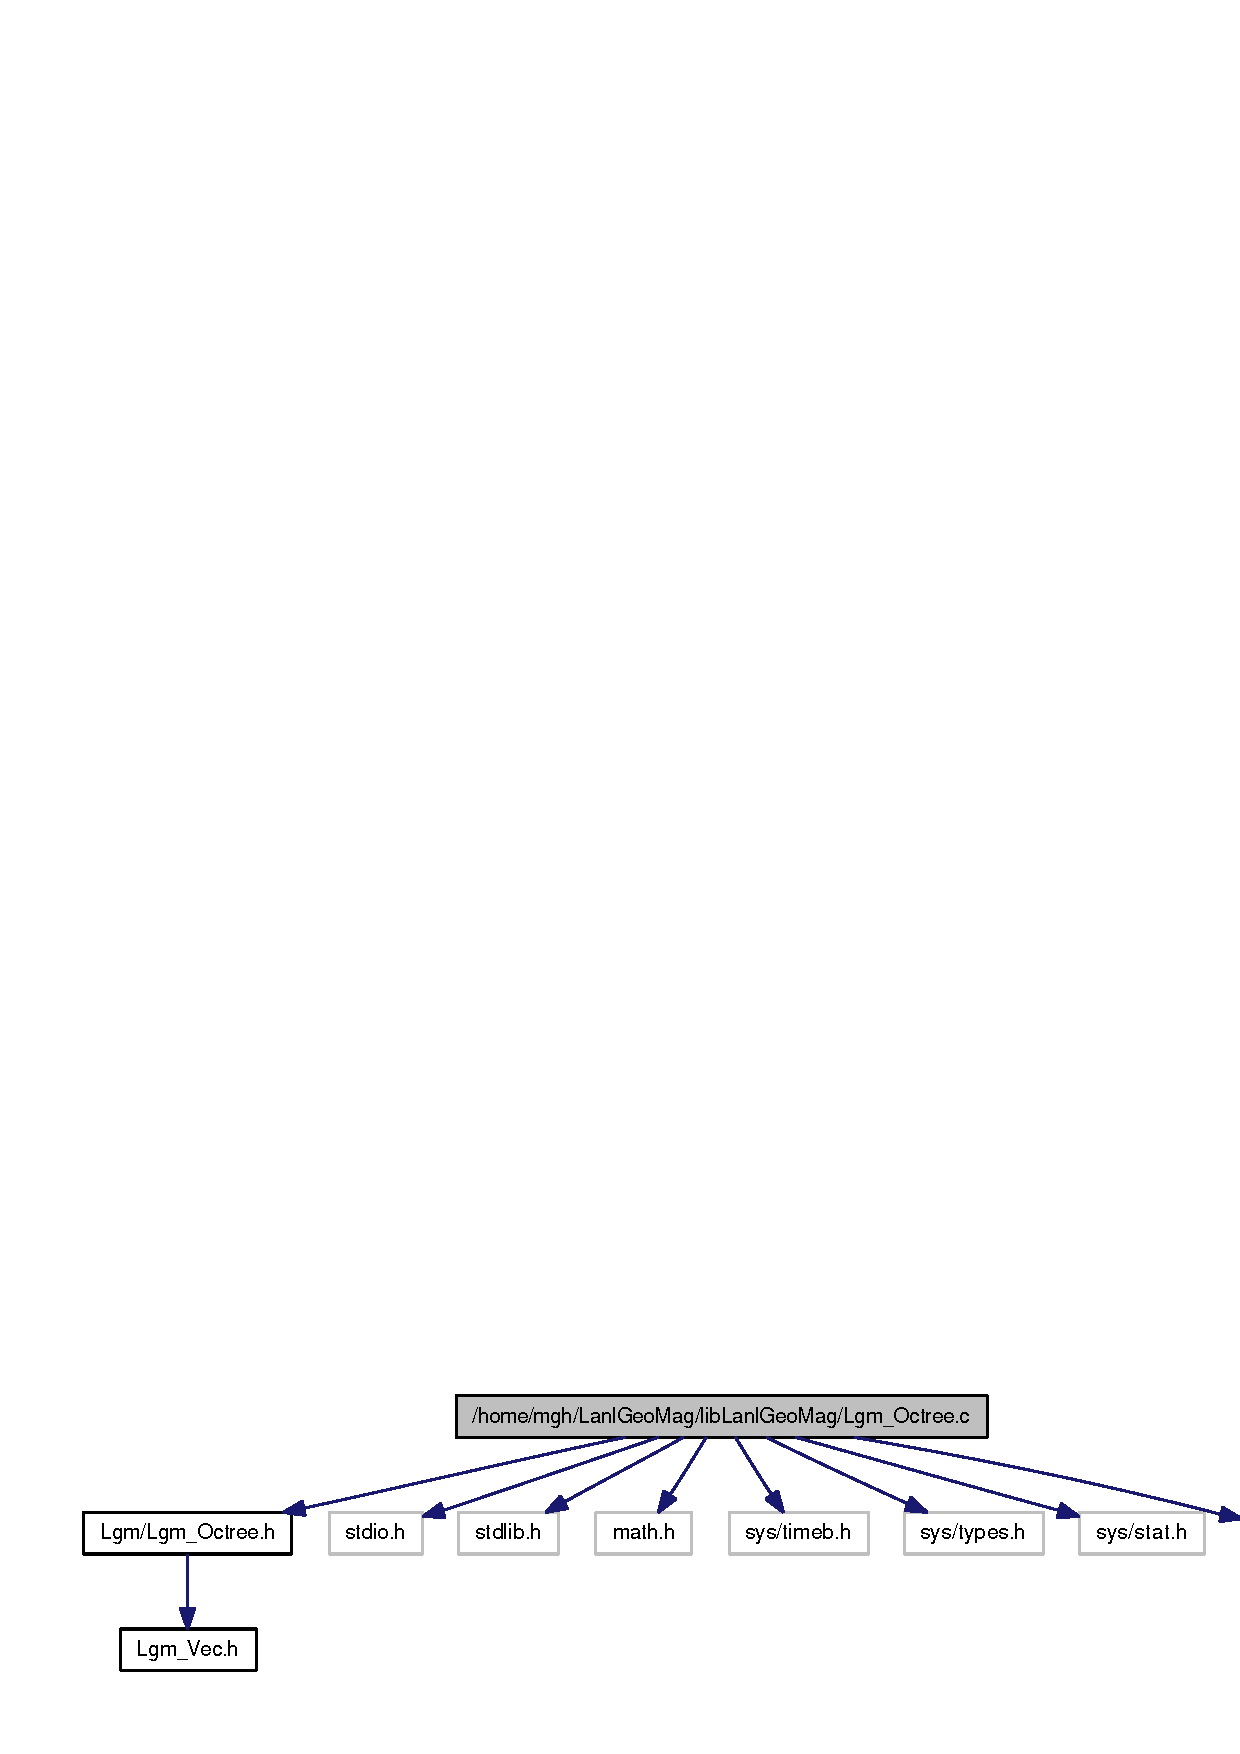
\includegraphics[width=321pt]{_lgm___octree_8c__incl}
\end{center}
\end{figure}
\subsection*{Functions}
\begin{CompactItemize}
\item 
double \hyperlink{_lgm___octree_8c_c350804981295b42e11e3e5978df415f}{ElapsedTime2} (struct timeb \hyperlink{_lgm___octree_8c_36c11daf675931ac69b5478131af8e27}{StartTime})
\item 
void \hyperlink{_lgm___octree_8c_5be6ddcd43586ee6989697d995319c31}{Binary} (unsigned int n, char $\ast$Str)
\item 
void \hyperlink{_lgm___octree_8c_ebbdef4a1addf536593f776187402c39}{Lgm\_\-OctreeFreeBranch} (\hyperlink{struct___lgm___octree_cell}{Lgm\_\-OctreeCell} $\ast$Cell)
\item 
void \hyperlink{_lgm___octree_8c_8966fb8ec73aa1c0e437604568685d13}{Lgm\_\-FreeOctree} (\hyperlink{struct___lgm___octree_cell}{Lgm\_\-OctreeCell} $\ast$ot)
\item 
\hyperlink{struct___lgm___octree_cell}{Lgm\_\-OctreeCell} $\ast$ \hyperlink{_lgm___octree_8c_cf7917181ce8b3f4ceb3f8f6af804889}{Lgm\_\-CreateOctreeRoot} ()
\item 
\hyperlink{struct___lgm___octree_cell}{Lgm\_\-OctreeCell} $\ast$ \hyperlink{_lgm___octree_8c_9b05a3600cfb54efc5f722928e1db5d4}{Lgm\_\-OctreeTraverseToLocCode} (\hyperlink{struct___lgm___octree_cell}{Lgm\_\-OctreeCell} $\ast$Cell, unsigned int ChildLevel, unsigned int xLocationCode, unsigned int yLocationCode, unsigned int zLocationCode)
\item 
\hyperlink{struct___lgm___octree_cell}{Lgm\_\-OctreeCell} $\ast$ \hyperlink{_lgm___octree_8c_271dd512841a7b4308c59db95853b8e1}{Lgm\_\-LocateNearestCell} (\hyperlink{struct___lgm___octree_cell}{Lgm\_\-OctreeCell} $\ast$Root, \hyperlink{struct_lgm___vector}{Lgm\_\-Vector} $\ast$q)
\item 
double \hyperlink{_lgm___octree_8c_07152ce3d1254cca2f4f2d4735de34b7}{MinDist} (\hyperlink{struct___lgm___octree_cell}{Lgm\_\-OctreeCell} $\ast$Cell, \hyperlink{struct_lgm___vector}{Lgm\_\-Vector} $\ast$q)
\item 
double \hyperlink{_lgm___octree_8c_cb735b055954d17d224db5a55dbd14e6}{InsertCell} (\hyperlink{struct___lgm___octree_cell}{Lgm\_\-OctreeCell} $\ast$Cell, \hyperlink{struct_lgm___vector}{Lgm\_\-Vector} $\ast$q, \hyperlink{struct__p_queue}{pQueue} $\ast$$\ast$PQ, double MaxDist2)
\item 
void \hyperlink{_lgm___octree_8c_0128a077b1023c02e79cfaf65a4e6cfc}{InsertPoint} (\hyperlink{struct___lgm___octree_cell}{Lgm\_\-OctreeCell} $\ast$Cell, int j, \hyperlink{struct_lgm___vector}{Lgm\_\-Vector} $\ast$q, \hyperlink{struct__p_queue}{pQueue} $\ast$$\ast$PQ)
\item 
\hyperlink{struct___lgm___octree_cell}{Lgm\_\-OctreeCell} $\ast$ \hyperlink{_lgm___octree_8c_9ff86b033bf330695e810d00ac8022e1}{DescendTowardClosestLeaf} (\hyperlink{struct___lgm___octree_cell}{Lgm\_\-OctreeCell} $\ast$Node, \hyperlink{struct__p_queue}{pQueue} $\ast$$\ast$PQ, \hyperlink{struct_lgm___vector}{Lgm\_\-Vector} $\ast$q, double MaxDist2)
\item 
void \hyperlink{_lgm___octree_8c_577327ba4885c8a45805115c03e606bd}{PrintPQ} (\hyperlink{struct__p_queue}{pQueue} $\ast$$\ast$PQ)
\item 
\hyperlink{struct__p_queue}{pQueue} $\ast$ \hyperlink{_lgm___octree_8c_653f08b2912abb5a5fb6c1761b8a8cec}{PopObj} (\hyperlink{struct__p_queue}{pQueue} $\ast$$\ast$PQ)
\item 
int \hyperlink{_lgm___octree_8c_885f0695706ada1ee750180afe105958}{Lgm\_\-Octree\_\-kNN} (\hyperlink{struct_lgm___vector}{Lgm\_\-Vector} $\ast$q, \hyperlink{struct___lgm___octree_cell}{Lgm\_\-OctreeCell} $\ast$Root, int K, int $\ast$Kgot, double MaxDist2, \hyperlink{struct___lgm___octree_data}{Lgm\_\-OctreeData} $\ast$kNN)
\item 
\hyperlink{struct___lgm___octree_cell}{Lgm\_\-OctreeCell} $\ast$ \hyperlink{_lgm___octree_8c_8faba8ef3514ee1be8aedd369afd4db9}{CreateNewOctants} (\hyperlink{struct___lgm___octree_cell}{Lgm\_\-OctreeCell} $\ast$Parent)
\item 
void \hyperlink{_lgm___octree_8c_3df40f5467250c1b9c2ba1053d38d76f}{SubDivideVolume} (\hyperlink{struct___lgm___octree_cell}{Lgm\_\-OctreeCell} $\ast$Vol)
\item 
void \hyperlink{_lgm___octree_8c_662a8337622fc6df46766be9249ec872}{Lgm\_\-OctreeScalePoint} (\hyperlink{struct_lgm___vector}{Lgm\_\-Vector} $\ast$u, \hyperlink{struct_lgm___vector}{Lgm\_\-Vector} $\ast$v, double Min, double Diff)
\item 
\hyperlink{struct___lgm___octree_cell}{Lgm\_\-OctreeCell} $\ast$ \hyperlink{_lgm___octree_8c_20080c6b6bf182550e7c1e99d3807020}{Lgm\_\-InitOctree} (\hyperlink{struct_lgm___vector}{Lgm\_\-Vector} $\ast$ObjectPoints, \hyperlink{struct_lgm___vector}{Lgm\_\-Vector} $\ast$ObjectData, unsigned long int N, double $\ast$Min, double $\ast$Max, double $\ast$Diff)
\end{CompactItemize}
\subsection*{Variables}
\begin{CompactItemize}
\item 
struct timeb \hyperlink{_lgm___octree_8c_36c11daf675931ac69b5478131af8e27}{StartTime}
\end{CompactItemize}


\subsection{Function Documentation}
\hypertarget{_lgm___octree_8c_c350804981295b42e11e3e5978df415f}{
\index{Lgm\_\-Octree.c@{Lgm\_\-Octree.c}!ElapsedTime2@{ElapsedTime2}}
\index{ElapsedTime2@{ElapsedTime2}!Lgm_Octree.c@{Lgm\_\-Octree.c}}
\subsubsection[{ElapsedTime2}]{\setlength{\rightskip}{0pt plus 5cm}double ElapsedTime2 (struct timeb {\em StartTime})}}
\label{_lgm___octree_8c_c350804981295b42e11e3e5978df415f}


\hypertarget{_lgm___octree_8c_5be6ddcd43586ee6989697d995319c31}{
\index{Lgm\_\-Octree.c@{Lgm\_\-Octree.c}!Binary@{Binary}}
\index{Binary@{Binary}!Lgm_Octree.c@{Lgm\_\-Octree.c}}
\subsubsection[{Binary}]{\setlength{\rightskip}{0pt plus 5cm}void Binary (unsigned int {\em n}, \/  char $\ast$ {\em Str})}}
\label{_lgm___octree_8c_5be6ddcd43586ee6989697d995319c31}




Definition at line 13 of file Lgm\_\-Octree.c.\hypertarget{_lgm___octree_8c_ebbdef4a1addf536593f776187402c39}{
\index{Lgm\_\-Octree.c@{Lgm\_\-Octree.c}!Lgm\_\-OctreeFreeBranch@{Lgm\_\-OctreeFreeBranch}}
\index{Lgm\_\-OctreeFreeBranch@{Lgm\_\-OctreeFreeBranch}!Lgm_Octree.c@{Lgm\_\-Octree.c}}
\subsubsection[{Lgm\_\-OctreeFreeBranch}]{\setlength{\rightskip}{0pt plus 5cm}void Lgm\_\-OctreeFreeBranch ({\bf Lgm\_\-OctreeCell} $\ast$ {\em Cell})}}
\label{_lgm___octree_8c_ebbdef4a1addf536593f776187402c39}




Definition at line 30 of file Lgm\_\-Octree.c.

Here is the call graph for this function:\nopagebreak
\begin{figure}[H]
\begin{center}
\leavevmode
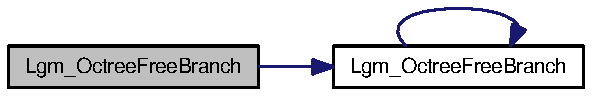
\includegraphics[width=160pt]{_lgm___octree_8c_ebbdef4a1addf536593f776187402c39_cgraph}
\end{center}
\end{figure}


Here is the caller graph for this function:\nopagebreak
\begin{figure}[H]
\begin{center}
\leavevmode
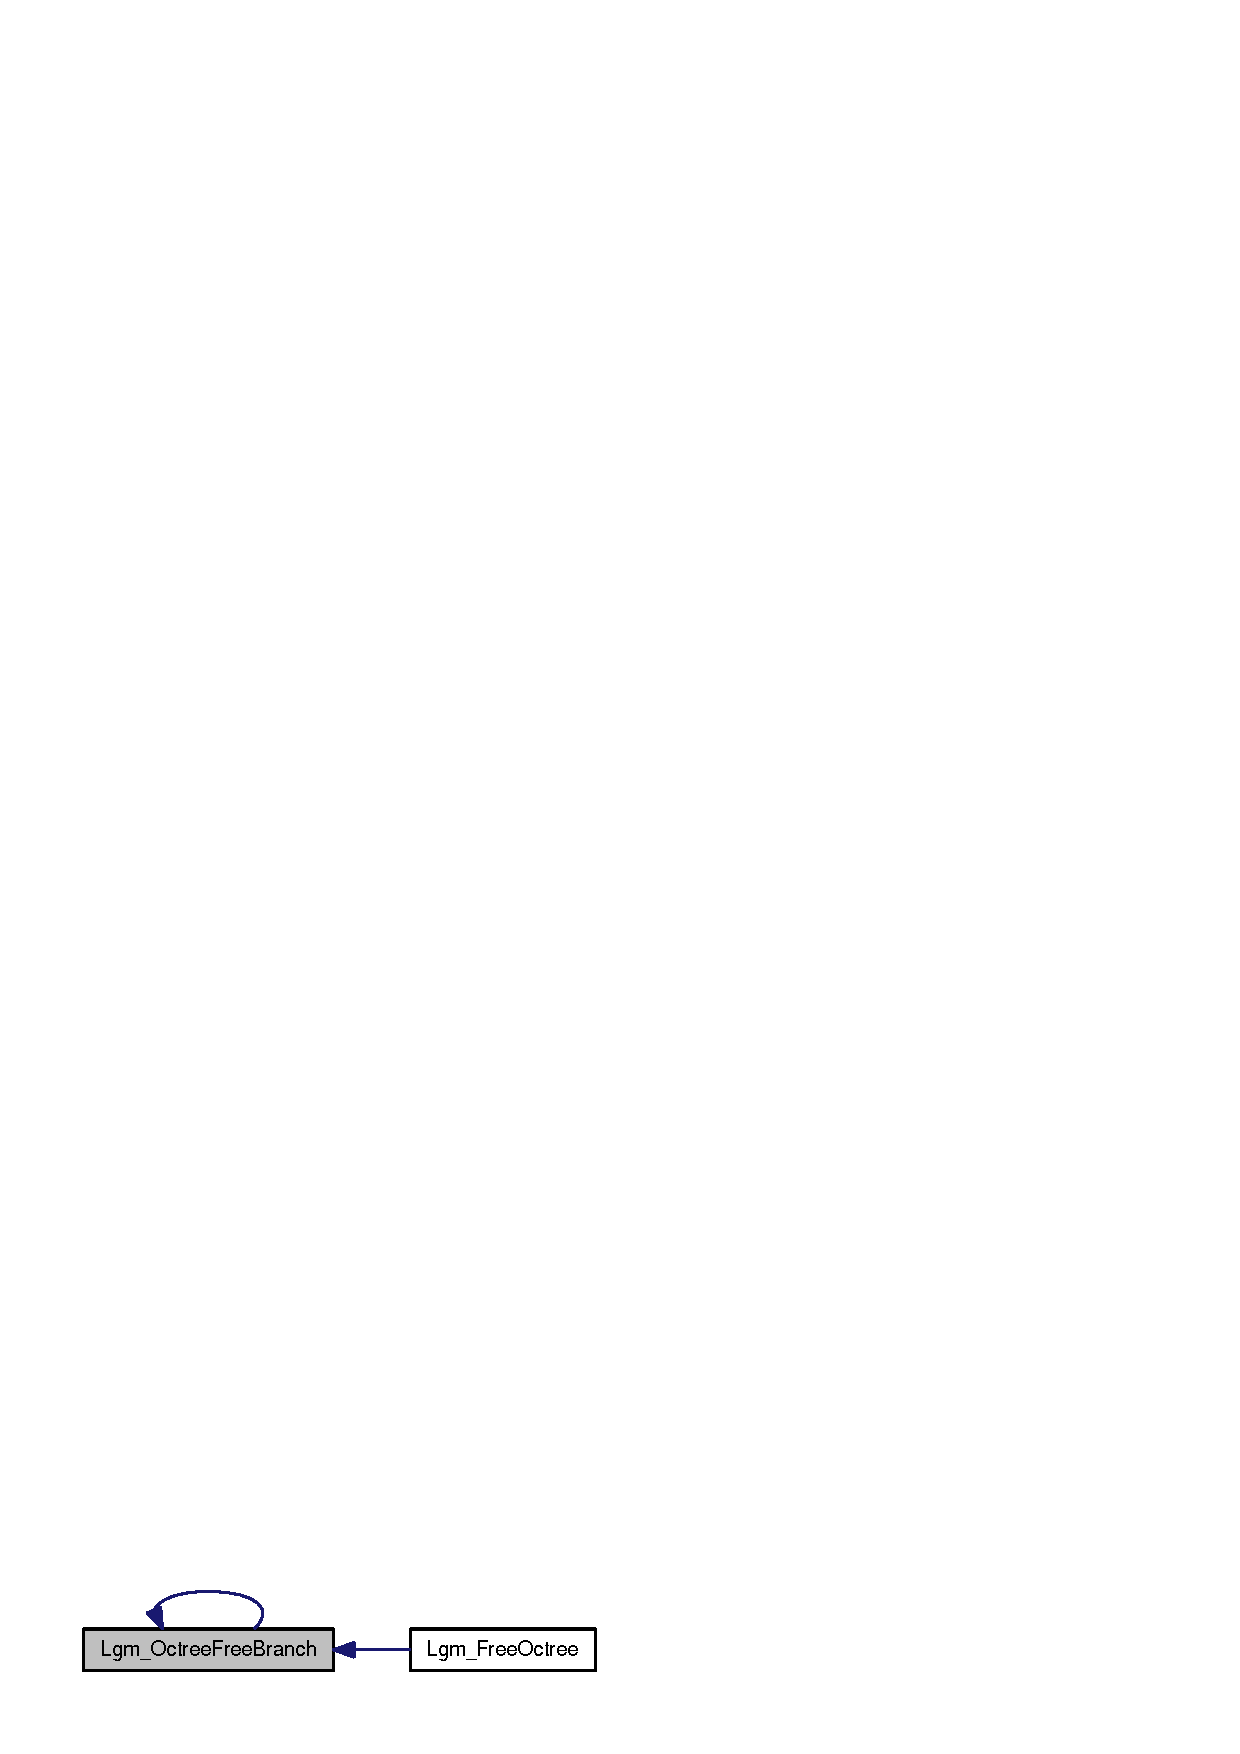
\includegraphics[width=145pt]{_lgm___octree_8c_ebbdef4a1addf536593f776187402c39_icgraph}
\end{center}
\end{figure}
\hypertarget{_lgm___octree_8c_8966fb8ec73aa1c0e437604568685d13}{
\index{Lgm\_\-Octree.c@{Lgm\_\-Octree.c}!Lgm\_\-FreeOctree@{Lgm\_\-FreeOctree}}
\index{Lgm\_\-FreeOctree@{Lgm\_\-FreeOctree}!Lgm_Octree.c@{Lgm\_\-Octree.c}}
\subsubsection[{Lgm\_\-FreeOctree}]{\setlength{\rightskip}{0pt plus 5cm}void Lgm\_\-FreeOctree ({\bf Lgm\_\-OctreeCell} $\ast$ {\em ot})}}
\label{_lgm___octree_8c_8966fb8ec73aa1c0e437604568685d13}




Definition at line 58 of file Lgm\_\-Octree.c.

Here is the call graph for this function:\nopagebreak
\begin{figure}[H]
\begin{center}
\leavevmode
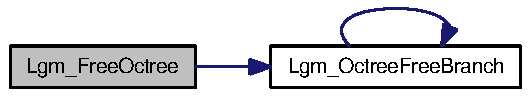
\includegraphics[width=145pt]{_lgm___octree_8c_8966fb8ec73aa1c0e437604568685d13_cgraph}
\end{center}
\end{figure}
\hypertarget{_lgm___octree_8c_cf7917181ce8b3f4ceb3f8f6af804889}{
\index{Lgm\_\-Octree.c@{Lgm\_\-Octree.c}!Lgm\_\-CreateOctreeRoot@{Lgm\_\-CreateOctreeRoot}}
\index{Lgm\_\-CreateOctreeRoot@{Lgm\_\-CreateOctreeRoot}!Lgm_Octree.c@{Lgm\_\-Octree.c}}
\subsubsection[{Lgm\_\-CreateOctreeRoot}]{\setlength{\rightskip}{0pt plus 5cm}{\bf Lgm\_\-OctreeCell}$\ast$ Lgm\_\-CreateOctreeRoot ()}}
\label{_lgm___octree_8c_cf7917181ce8b3f4ceb3f8f6af804889}




Definition at line 64 of file Lgm\_\-Octree.c.

Here is the caller graph for this function:\nopagebreak
\begin{figure}[H]
\begin{center}
\leavevmode
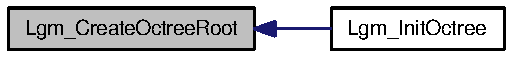
\includegraphics[width=141pt]{_lgm___octree_8c_cf7917181ce8b3f4ceb3f8f6af804889_icgraph}
\end{center}
\end{figure}
\hypertarget{_lgm___octree_8c_9b05a3600cfb54efc5f722928e1db5d4}{
\index{Lgm\_\-Octree.c@{Lgm\_\-Octree.c}!Lgm\_\-OctreeTraverseToLocCode@{Lgm\_\-OctreeTraverseToLocCode}}
\index{Lgm\_\-OctreeTraverseToLocCode@{Lgm\_\-OctreeTraverseToLocCode}!Lgm_Octree.c@{Lgm\_\-Octree.c}}
\subsubsection[{Lgm\_\-OctreeTraverseToLocCode}]{\setlength{\rightskip}{0pt plus 5cm}{\bf Lgm\_\-OctreeCell}$\ast$ Lgm\_\-OctreeTraverseToLocCode ({\bf Lgm\_\-OctreeCell} $\ast$ {\em Cell}, \/  unsigned int {\em ChildLevel}, \/  unsigned int {\em xLocationCode}, \/  unsigned int {\em yLocationCode}, \/  unsigned int {\em zLocationCode})}}
\label{_lgm___octree_8c_9b05a3600cfb54efc5f722928e1db5d4}




Definition at line 99 of file Lgm\_\-Octree.c.

Here is the caller graph for this function:\nopagebreak
\begin{figure}[H]
\begin{center}
\leavevmode
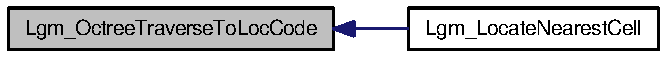
\includegraphics[width=178pt]{_lgm___octree_8c_9b05a3600cfb54efc5f722928e1db5d4_icgraph}
\end{center}
\end{figure}
\hypertarget{_lgm___octree_8c_271dd512841a7b4308c59db95853b8e1}{
\index{Lgm\_\-Octree.c@{Lgm\_\-Octree.c}!Lgm\_\-LocateNearestCell@{Lgm\_\-LocateNearestCell}}
\index{Lgm\_\-LocateNearestCell@{Lgm\_\-LocateNearestCell}!Lgm_Octree.c@{Lgm\_\-Octree.c}}
\subsubsection[{Lgm\_\-LocateNearestCell}]{\setlength{\rightskip}{0pt plus 5cm}{\bf Lgm\_\-OctreeCell}$\ast$ Lgm\_\-LocateNearestCell ({\bf Lgm\_\-OctreeCell} $\ast$ {\em Root}, \/  {\bf Lgm\_\-Vector} $\ast$ {\em q})}}
\label{_lgm___octree_8c_271dd512841a7b4308c59db95853b8e1}




Definition at line 127 of file Lgm\_\-Octree.c.

Here is the call graph for this function:\nopagebreak
\begin{figure}[H]
\begin{center}
\leavevmode
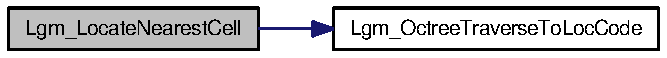
\includegraphics[width=178pt]{_lgm___octree_8c_271dd512841a7b4308c59db95853b8e1_cgraph}
\end{center}
\end{figure}
\hypertarget{_lgm___octree_8c_07152ce3d1254cca2f4f2d4735de34b7}{
\index{Lgm\_\-Octree.c@{Lgm\_\-Octree.c}!MinDist@{MinDist}}
\index{MinDist@{MinDist}!Lgm_Octree.c@{Lgm\_\-Octree.c}}
\subsubsection[{MinDist}]{\setlength{\rightskip}{0pt plus 5cm}double MinDist ({\bf Lgm\_\-OctreeCell} $\ast$ {\em Cell}, \/  {\bf Lgm\_\-Vector} $\ast$ {\em q})}}
\label{_lgm___octree_8c_07152ce3d1254cca2f4f2d4735de34b7}




Definition at line 162 of file Lgm\_\-Octree.c.

Here is the caller graph for this function:\nopagebreak
\begin{figure}[H]
\begin{center}
\leavevmode
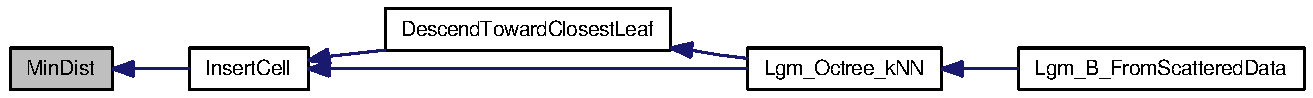
\includegraphics[width=333pt]{_lgm___octree_8c_07152ce3d1254cca2f4f2d4735de34b7_icgraph}
\end{center}
\end{figure}
\hypertarget{_lgm___octree_8c_cb735b055954d17d224db5a55dbd14e6}{
\index{Lgm\_\-Octree.c@{Lgm\_\-Octree.c}!InsertCell@{InsertCell}}
\index{InsertCell@{InsertCell}!Lgm_Octree.c@{Lgm\_\-Octree.c}}
\subsubsection[{InsertCell}]{\setlength{\rightskip}{0pt plus 5cm}double InsertCell ({\bf Lgm\_\-OctreeCell} $\ast$ {\em Cell}, \/  {\bf Lgm\_\-Vector} $\ast$ {\em q}, \/  {\bf pQueue} $\ast$$\ast$ {\em PQ}, \/  double {\em MaxDist2})}}
\label{_lgm___octree_8c_cb735b055954d17d224db5a55dbd14e6}




Definition at line 198 of file Lgm\_\-Octree.c.

Here is the call graph for this function:\nopagebreak
\begin{figure}[H]
\begin{center}
\leavevmode
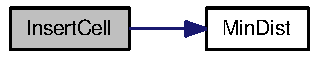
\includegraphics[width=94pt]{_lgm___octree_8c_cb735b055954d17d224db5a55dbd14e6_cgraph}
\end{center}
\end{figure}


Here is the caller graph for this function:\nopagebreak
\begin{figure}[H]
\begin{center}
\leavevmode
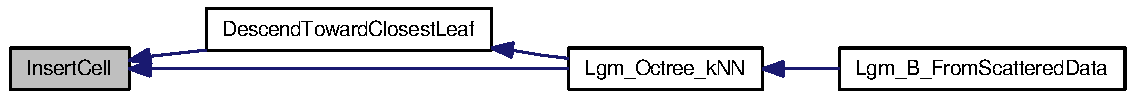
\includegraphics[width=290pt]{_lgm___octree_8c_cb735b055954d17d224db5a55dbd14e6_icgraph}
\end{center}
\end{figure}
\hypertarget{_lgm___octree_8c_0128a077b1023c02e79cfaf65a4e6cfc}{
\index{Lgm\_\-Octree.c@{Lgm\_\-Octree.c}!InsertPoint@{InsertPoint}}
\index{InsertPoint@{InsertPoint}!Lgm_Octree.c@{Lgm\_\-Octree.c}}
\subsubsection[{InsertPoint}]{\setlength{\rightskip}{0pt plus 5cm}void InsertPoint ({\bf Lgm\_\-OctreeCell} $\ast$ {\em Cell}, \/  int {\em j}, \/  {\bf Lgm\_\-Vector} $\ast$ {\em q}, \/  {\bf pQueue} $\ast$$\ast$ {\em PQ})}}
\label{_lgm___octree_8c_0128a077b1023c02e79cfaf65a4e6cfc}




Definition at line 282 of file Lgm\_\-Octree.c.

Here is the caller graph for this function:\nopagebreak
\begin{figure}[H]
\begin{center}
\leavevmode
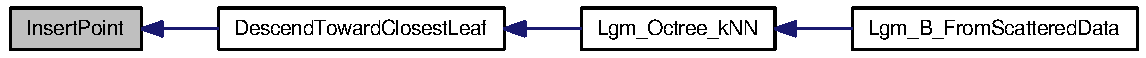
\includegraphics[width=293pt]{_lgm___octree_8c_0128a077b1023c02e79cfaf65a4e6cfc_icgraph}
\end{center}
\end{figure}
\hypertarget{_lgm___octree_8c_9ff86b033bf330695e810d00ac8022e1}{
\index{Lgm\_\-Octree.c@{Lgm\_\-Octree.c}!DescendTowardClosestLeaf@{DescendTowardClosestLeaf}}
\index{DescendTowardClosestLeaf@{DescendTowardClosestLeaf}!Lgm_Octree.c@{Lgm\_\-Octree.c}}
\subsubsection[{DescendTowardClosestLeaf}]{\setlength{\rightskip}{0pt plus 5cm}{\bf Lgm\_\-OctreeCell}$\ast$ DescendTowardClosestLeaf ({\bf Lgm\_\-OctreeCell} $\ast$ {\em Node}, \/  {\bf pQueue} $\ast$$\ast$ {\em PQ}, \/  {\bf Lgm\_\-Vector} $\ast$ {\em q}, \/  double {\em MaxDist2})}}
\label{_lgm___octree_8c_9ff86b033bf330695e810d00ac8022e1}




Definition at line 350 of file Lgm\_\-Octree.c.

Here is the call graph for this function:\nopagebreak
\begin{figure}[H]
\begin{center}
\leavevmode
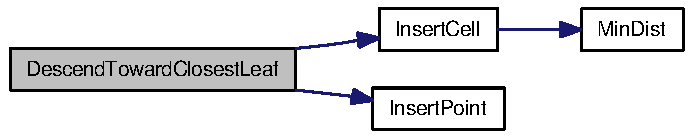
\includegraphics[width=184pt]{_lgm___octree_8c_9ff86b033bf330695e810d00ac8022e1_cgraph}
\end{center}
\end{figure}


Here is the caller graph for this function:\nopagebreak
\begin{figure}[H]
\begin{center}
\leavevmode
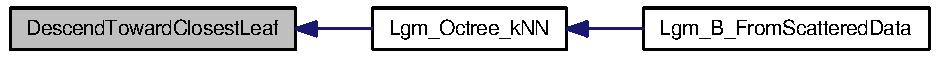
\includegraphics[width=243pt]{_lgm___octree_8c_9ff86b033bf330695e810d00ac8022e1_icgraph}
\end{center}
\end{figure}
\hypertarget{_lgm___octree_8c_577327ba4885c8a45805115c03e606bd}{
\index{Lgm\_\-Octree.c@{Lgm\_\-Octree.c}!PrintPQ@{PrintPQ}}
\index{PrintPQ@{PrintPQ}!Lgm_Octree.c@{Lgm\_\-Octree.c}}
\subsubsection[{PrintPQ}]{\setlength{\rightskip}{0pt plus 5cm}void PrintPQ ({\bf pQueue} $\ast$$\ast$ {\em PQ})}}
\label{_lgm___octree_8c_577327ba4885c8a45805115c03e606bd}




Definition at line 399 of file Lgm\_\-Octree.c.\hypertarget{_lgm___octree_8c_653f08b2912abb5a5fb6c1761b8a8cec}{
\index{Lgm\_\-Octree.c@{Lgm\_\-Octree.c}!PopObj@{PopObj}}
\index{PopObj@{PopObj}!Lgm_Octree.c@{Lgm\_\-Octree.c}}
\subsubsection[{PopObj}]{\setlength{\rightskip}{0pt plus 5cm}{\bf pQueue}$\ast$ PopObj ({\bf pQueue} $\ast$$\ast$ {\em PQ})}}
\label{_lgm___octree_8c_653f08b2912abb5a5fb6c1761b8a8cec}




Definition at line 423 of file Lgm\_\-Octree.c.

Here is the caller graph for this function:\nopagebreak
\begin{figure}[H]
\begin{center}
\leavevmode
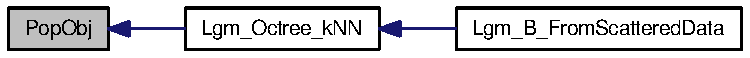
\includegraphics[width=198pt]{_lgm___octree_8c_653f08b2912abb5a5fb6c1761b8a8cec_icgraph}
\end{center}
\end{figure}
\hypertarget{_lgm___octree_8c_885f0695706ada1ee750180afe105958}{
\index{Lgm\_\-Octree.c@{Lgm\_\-Octree.c}!Lgm\_\-Octree\_\-kNN@{Lgm\_\-Octree\_\-kNN}}
\index{Lgm\_\-Octree\_\-kNN@{Lgm\_\-Octree\_\-kNN}!Lgm_Octree.c@{Lgm\_\-Octree.c}}
\subsubsection[{Lgm\_\-Octree\_\-kNN}]{\setlength{\rightskip}{0pt plus 5cm}int Lgm\_\-Octree\_\-kNN ({\bf Lgm\_\-Vector} $\ast$ {\em q}, \/  {\bf Lgm\_\-OctreeCell} $\ast$ {\em Root}, \/  int {\em K}, \/  int $\ast$ {\em Kgot}, \/  double {\em MaxDist2}, \/  {\bf Lgm\_\-OctreeData} $\ast$ {\em kNN})}}
\label{_lgm___octree_8c_885f0695706ada1ee750180afe105958}




Definition at line 474 of file Lgm\_\-Octree.c.

Here is the call graph for this function:\nopagebreak
\begin{figure}[H]
\begin{center}
\leavevmode
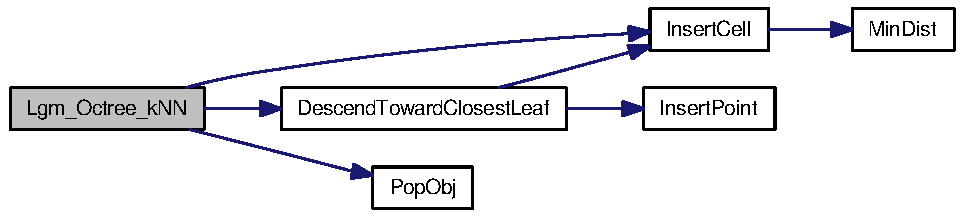
\includegraphics[width=249pt]{_lgm___octree_8c_885f0695706ada1ee750180afe105958_cgraph}
\end{center}
\end{figure}


Here is the caller graph for this function:\nopagebreak
\begin{figure}[H]
\begin{center}
\leavevmode
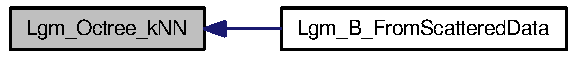
\includegraphics[width=156pt]{_lgm___octree_8c_885f0695706ada1ee750180afe105958_icgraph}
\end{center}
\end{figure}
\hypertarget{_lgm___octree_8c_8faba8ef3514ee1be8aedd369afd4db9}{
\index{Lgm\_\-Octree.c@{Lgm\_\-Octree.c}!CreateNewOctants@{CreateNewOctants}}
\index{CreateNewOctants@{CreateNewOctants}!Lgm_Octree.c@{Lgm\_\-Octree.c}}
\subsubsection[{CreateNewOctants}]{\setlength{\rightskip}{0pt plus 5cm}{\bf Lgm\_\-OctreeCell}$\ast$ CreateNewOctants ({\bf Lgm\_\-OctreeCell} $\ast$ {\em Parent})}}
\label{_lgm___octree_8c_8faba8ef3514ee1be8aedd369afd4db9}




Definition at line 585 of file Lgm\_\-Octree.c.

Here is the caller graph for this function:\nopagebreak
\begin{figure}[H]
\begin{center}
\leavevmode
\includegraphics[width=196pt]{_lgm___octree_8c_8faba8ef3514ee1be8aedd369afd4db9_icgraph}
\end{center}
\end{figure}
\hypertarget{_lgm___octree_8c_3df40f5467250c1b9c2ba1053d38d76f}{
\index{Lgm\_\-Octree.c@{Lgm\_\-Octree.c}!SubDivideVolume@{SubDivideVolume}}
\index{SubDivideVolume@{SubDivideVolume}!Lgm_Octree.c@{Lgm\_\-Octree.c}}
\subsubsection[{SubDivideVolume}]{\setlength{\rightskip}{0pt plus 5cm}void SubDivideVolume ({\bf Lgm\_\-OctreeCell} $\ast$ {\em Vol})}}
\label{_lgm___octree_8c_3df40f5467250c1b9c2ba1053d38d76f}




Definition at line 654 of file Lgm\_\-Octree.c.

Here is the call graph for this function:\nopagebreak
\begin{figure}[H]
\begin{center}
\leavevmode
\includegraphics[width=201pt]{_lgm___octree_8c_3df40f5467250c1b9c2ba1053d38d76f_cgraph}
\end{center}
\end{figure}


Here is the caller graph for this function:\nopagebreak
\begin{figure}[H]
\begin{center}
\leavevmode
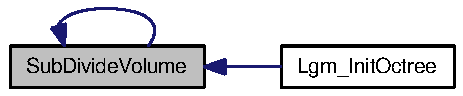
\includegraphics[width=129pt]{_lgm___octree_8c_3df40f5467250c1b9c2ba1053d38d76f_icgraph}
\end{center}
\end{figure}
\hypertarget{_lgm___octree_8c_662a8337622fc6df46766be9249ec872}{
\index{Lgm\_\-Octree.c@{Lgm\_\-Octree.c}!Lgm\_\-OctreeScalePoint@{Lgm\_\-OctreeScalePoint}}
\index{Lgm\_\-OctreeScalePoint@{Lgm\_\-OctreeScalePoint}!Lgm_Octree.c@{Lgm\_\-Octree.c}}
\subsubsection[{Lgm\_\-OctreeScalePoint}]{\setlength{\rightskip}{0pt plus 5cm}void Lgm\_\-OctreeScalePoint ({\bf Lgm\_\-Vector} $\ast$ {\em u}, \/  {\bf Lgm\_\-Vector} $\ast$ {\em v}, \/  double {\em Min}, \/  double {\em Diff})}}
\label{_lgm___octree_8c_662a8337622fc6df46766be9249ec872}




Definition at line 740 of file Lgm\_\-Octree.c.\hypertarget{_lgm___octree_8c_20080c6b6bf182550e7c1e99d3807020}{
\index{Lgm\_\-Octree.c@{Lgm\_\-Octree.c}!Lgm\_\-InitOctree@{Lgm\_\-InitOctree}}
\index{Lgm\_\-InitOctree@{Lgm\_\-InitOctree}!Lgm_Octree.c@{Lgm\_\-Octree.c}}
\subsubsection[{Lgm\_\-InitOctree}]{\setlength{\rightskip}{0pt plus 5cm}{\bf Lgm\_\-OctreeCell}$\ast$ Lgm\_\-InitOctree ({\bf Lgm\_\-Vector} $\ast$ {\em ObjectPoints}, \/  {\bf Lgm\_\-Vector} $\ast$ {\em ObjectData}, \/  unsigned long int {\em N}, \/  double $\ast$ {\em Min}, \/  double $\ast$ {\em Max}, \/  double $\ast$ {\em Diff})}}
\label{_lgm___octree_8c_20080c6b6bf182550e7c1e99d3807020}




Definition at line 767 of file Lgm\_\-Octree.c.

Here is the call graph for this function:\nopagebreak
\begin{figure}[H]
\begin{center}
\leavevmode
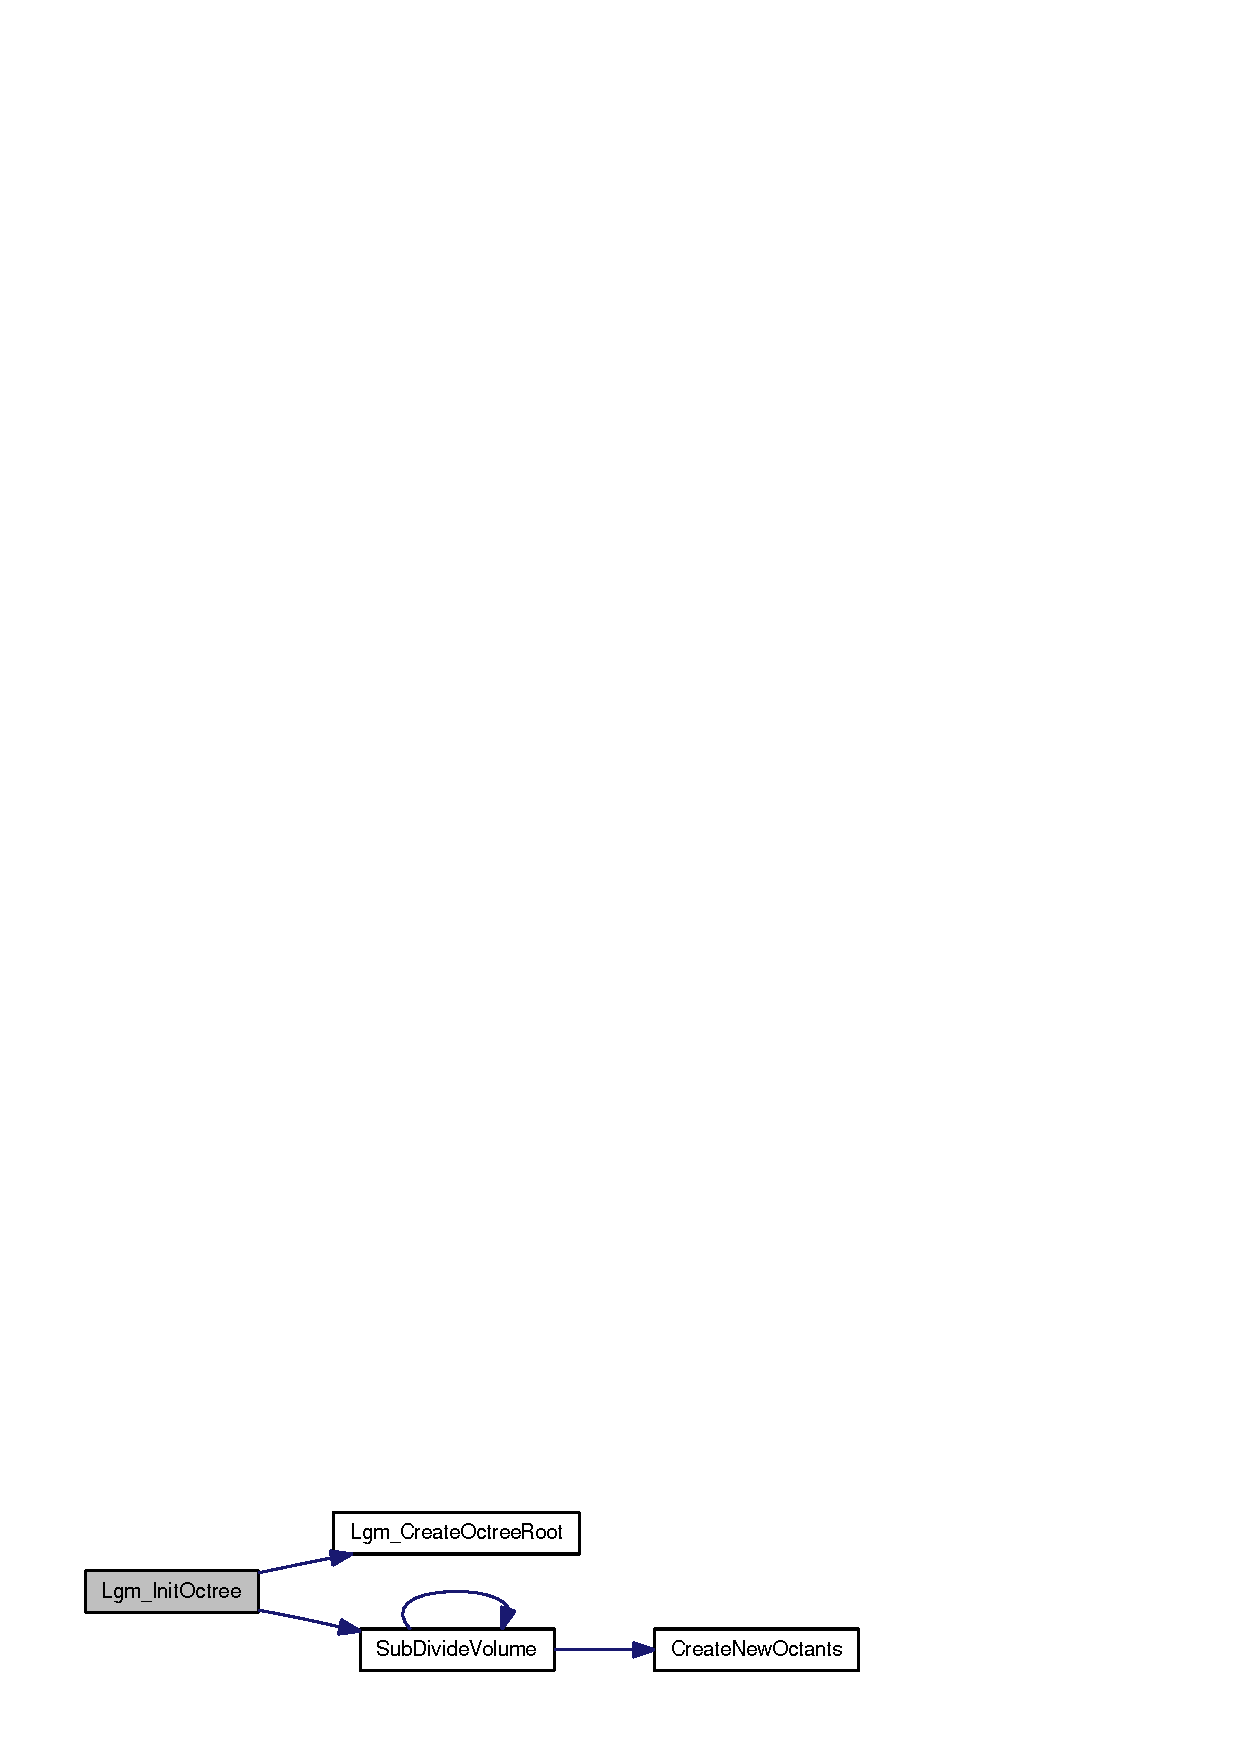
\includegraphics[width=208pt]{_lgm___octree_8c_20080c6b6bf182550e7c1e99d3807020_cgraph}
\end{center}
\end{figure}


\subsection{Variable Documentation}
\hypertarget{_lgm___octree_8c_36c11daf675931ac69b5478131af8e27}{
\index{Lgm\_\-Octree.c@{Lgm\_\-Octree.c}!StartTime@{StartTime}}
\index{StartTime@{StartTime}!Lgm_Octree.c@{Lgm\_\-Octree.c}}
\subsubsection[{StartTime}]{\setlength{\rightskip}{0pt plus 5cm}struct timeb {\bf StartTime}}}
\label{_lgm___octree_8c_36c11daf675931ac69b5478131af8e27}




Definition at line 10 of file Lgm\_\-Octree.c.